\section{Consistency Failure Analysis}
\label{sec:failures}

This section localizes failures under the frozen Qwen condition and contrasts them with symbolic error patterns. Counts refer to bundles with at least one violation in a family unless noted.

\subsection{Qwen: widespread multiple violations}

For all four Qwen systems, \textbf{transition} constraints fail on \textbf{192/192} bundles in the H4 subset. Failures are not explained by a single rare constraint on an otherwise consistent bundle:

\begin{table}[t]
\centering
\caption{Qwen violation multiplicity (H4; frozen).}
\label{tab:violations}
\begin{tabular}{lrrr}
\toprule
System & Mean viol./bundle & Frac.\ exactly one & Frac.\ multiple \\
\midrule
B1 compact & 3.59 & 0.031 & 0.969 \\
B3 recency & 3.59 & 0.031 & 0.969 \\
B4 BM25 & 3.33 & 0.177 & 0.823 \\
H0 reference & 3.50 & 0.000 & 1.000 \\
\bottomrule
\end{tabular}
\end{table}

\textbf{BCR~$=$~0} under Qwen therefore reflects \textbf{widespread multi-constraint inconsistency}, not one recurring isolated miss.

\subsection{Constraint families (Qwen)}

Family hit counts (bundles with $\ge 1$ failure) and violation rates are reported in Figure~\ref{fig:constraints} and Table~\ref{tab:constraints}; query-family Acc appears in Table~\ref{tab:queryfam} (Appendix~\ref{app:extrafigs}). Transition and provenance dominate. H0 reduces uniqueness hits to zero in this snapshot but \textbf{increases} contradiction hits and still fails every transition constraint. B4 reduces provenance hits relative to B1/B3, aligning with its higher CSR.

\begin{figure}[t]
\centering
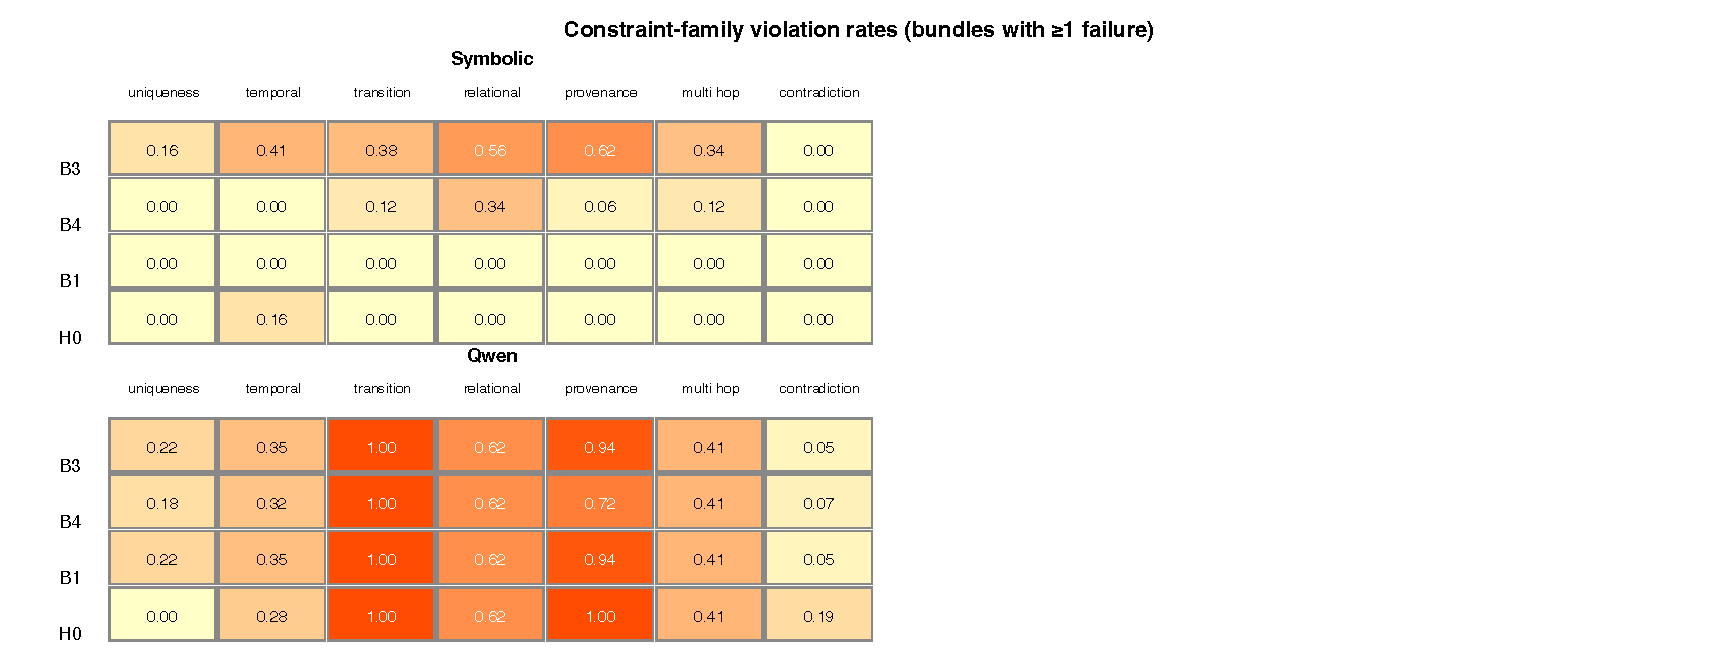
\includegraphics[width=\linewidth]{figures/fig4-constraint-family-heatmap.pdf}
\caption{Constraint-family violation rates under symbolic and Qwen readers.}
\label{fig:constraints}
\end{figure}

\subsection{Abstention and malformed output}

Qwen abstention is high for B1/B3 (0.728), lower for B4 (0.579) and H0 (0.483). Malformed rates remain low for flats/BM25 ($\le$0.007) and higher for H0 (0.029). Lower abstention with higher Acc under H0 does not restore BCR; some additional answered queries still violate joint constraints (near-zero Acc--CSR correlation).

\subsection{Evidence availability versus reader composition}

Symbolic BM25 and H0 can place correct evidence in scope and still show Acc--BCR gaps; under Qwen, error decomposition emphasizes \textbf{reader composition} failures even when retrieval improves Acc. Frozen H4 notes include non-zero reader-failure-on-correct-evidence rates. The methodological implication suggested by the decomposition is consistent with the observed pattern that improving evidence can shift Acc without necessarily restoring $\Phi=1$ under this frozen evaluation pipeline.

\subsection{Symbolic contrast (brief)}

Under the deterministic reader, family Acc and BCR are much higher; gaps concentrate on retrieval/capacity regimes (e.g., recency) rather than universal transition collapse. Ablations link archive/temporal/graph components to family Acc drops. This contrast indicates that Qwen BCR flooring is reader-regime-specific, not a claim that the constraint suite is unsatisfiable in principle (gold and strong symbolic systems achieve BCR~$=$~1).
